\documentclass[11pt,a4paper]{article}

% ---------------------------------------------------------------------------
% Packages (all standard; compiles on Overleaf and with TeX Live
% texlive-latex-recommended + texlive-latex-extra + texlive-pictures)
% ---------------------------------------------------------------------------
\usepackage[margin=2.3cm]{geometry}
\usepackage[T1]{fontenc}
\usepackage[utf8]{inputenc}
\usepackage{lmodern}
\usepackage{microtype}
\usepackage{amsmath,amssymb}
\usepackage{graphicx}
\usepackage{booktabs}
\usepackage{multirow}
\usepackage{array}
\usepackage{xcolor}
\usepackage{enumitem}
\usepackage{caption}
\usepackage{float}
\usepackage{listings}
\usepackage{tikz}
\usetikzlibrary{arrows.meta,positioning}
\usepackage[colorlinks=true,linkcolor=blue!50!black,citecolor=blue!50!black,urlcolor=blue!50!black]{hyperref}

\graphicspath{{figures/}}
\setlist{itemsep=2pt,topsep=4pt}
\captionsetup{font=small,labelfont=bf}

\lstset{basicstyle=\ttfamily\footnotesize,breaklines=true,frame=single,
        framerule=0.3pt,rulecolor=\color{gray!60},backgroundcolor=\color{gray!6},
        columns=fullflexible,keepspaces=true}

\newcommand{\gd}{\text{GD}}
\newcommand{\gdw}{\text{GD-W}}
\newcommand{\gdd}{\text{GD-D}}
\newcommand{\gdh}{\text{GD-H}}
\newcommand{\code}[1]{\texttt{#1}}

% ---------------------------------------------------------------------------
\title{\textbf{Reproducing and Extending Greedy-Dual Keep-Alive\\for Serverless Cold-Start Mitigation}\\[4pt]
\large Course Project Report --- Cloud Computing, IIT Delhi}

% TODO: replace the placeholders below with the authors' names and entry numbers.
\author{
  Author Name 1 \quad (Entry No.) \\
  Author Name 2 \quad (Entry No.) \\
  Author Name 3 \quad (Entry No.) \\
  Author Name 4 \quad (Entry No.)
}
\date{November 2026}

\begin{document}
\maketitle

% ===========================================================================
\begin{abstract}
Serverless (Function-as-a-Service) platforms keep function containers ``warm'' in memory
to avoid cold-start latency, and must decide which containers to evict when memory runs out.
FaasCache~\cite{fuerst2021faascache} showed that this keep-alive problem is equivalent to
object caching and proposed a Greedy-Dual (\gd{}) policy that weights each container by
access frequency, cold-start cost and memory size. We reproduce FaasCache's central result
with the authors' own simulator on the real Azure Functions 2019 trace~\cite{shahrad2020serverless}:
\gd{} incurs about $3\times$ less cold-start overhead than the fixed-timeout (TTL) policy
used in production platforms at 8\,GB of server memory, and the result holds across three
independently sampled traces. Along the way we document two issues in the published artifact
that silently invalidate a naive reproduction: (i) a naively sampled trace contains functions
whose concurrent, non-evictable running containers exceed any realistic server, which makes
every policy look identical; and (ii) the artifact's analysis script interprets the
simulator's two timing fields the opposite way from the simulator itself. We then extend \gd{}
with three variants that each change one aspect of its frequency term: weighting (\gdw{}),
ageing (\gdd{}) and persistence across evictions (\gdh{}). After screening 16
configurations and validating the best of each on three trace seeds, \gdw{} with a squared
cost term reduces cold-start overhead by a further 9--17\% relative to \gd{}, beating it on
every seed at every memory size from 4\,GB upwards. A per-function breakdown shows why: \gdw{}
accepts \emph{more} cold starts on cheap functions in exchange for fewer cold starts on the
most expensive quartile of functions, which carries 80--90\% of all cold-start time.
Frequency decay and persistence give no reliable improvement.
\end{abstract}

\tableofcontents
\newpage

% ===========================================================================
\section{Introduction}
\label{sec:intro}

In Function-as-a-Service (FaaS) platforms such as AWS Lambda, Azure Functions and
Google Cloud Functions, developers upload individual functions and the provider runs
them on demand inside isolated containers. When a request arrives and no initialised
container of that function exists, the platform must start one --- launching the
sandbox, loading the language runtime, importing dependencies and running
initialisation code. This \emph{cold start} can take from hundreds of milliseconds to
many seconds, often far longer than the function's own execution time. Once a container
has served a request it can be kept \emph{warm} in memory so that the next request runs
immediately, but warm containers occupy server memory even while idle.

Every FaaS platform therefore needs a \emph{keep-alive policy}: which idle containers to
keep, and which to terminate when memory is needed for new ones. Production platforms
largely use a fixed time-to-live (TTL): a container is kept for a fixed period (e.g.\ 10
minutes) after its last use and then discarded, regardless of how popular, large or
expensive to restart its function is.

Fuerst and Sharma's FaasCache~\cite{fuerst2021faascache} observes that keep-alive is an
instance of \emph{object caching}: warm containers are cached objects, a cold start is a
cache miss, the cold-start time is the miss cost, and the container's memory footprint is
the object size. This lets decades of caching research be applied directly. In particular,
they adapt the Greedy-Dual-Size-Frequency family of algorithms~\cite{cao1997gds,cherkasova1998gdsf}
into a keep-alive policy (\gd{}) and report that it substantially reduces cold-start overhead
compared with TTL.

\paragraph{Goals.} This project has two goals:
\begin{enumerate}
  \item \textbf{Reproduce} FaasCache's central result --- that \gd{} beats TTL and other
        keep-alive policies on cold-start overhead --- using the authors' open-source
        simulator~\cite{faascachesim} and the real Azure Functions trace~\cite{azuredataset2019}.
  \item \textbf{Extend} \gd{} with a concrete new idea, evaluate it the same way, and
        explain the outcome.
\end{enumerate}

\paragraph{Contributions.}
\begin{itemize}
  \item A working, documented reproduction pipeline (trace generation, simulation sweeps,
        analysis and figures) on a modest 8-core / 8\,GB virtual machine, with all patches
        needed to run the 2021 artifact on a modern Python stack.
  \item Reproduction of the headline result: \gd{} has $\approx\!3\times$ lower cold-start
        overhead than TTL at 8\,GB, growing to $\approx\!9\times$ at 16\,GB, robust across
        three independently sampled traces (Section~\ref{sec:baseline}).
  \item Two methodological findings about the artifact (Section~\ref{sec:pitfalls}): a
        trace-sampling pathology that makes all policies indistinguishable, with a principled
        footprint filter that fixes it; and an inverted latency metric in the analysis
        script, with a corrected metric consistent with the simulator.
  \item Three \gd{} variants that each change one aspect of the frequency term, validated by
        exact-equivalence tests, screened over 16 configurations and confirmed on three trace
        seeds (Sections~\ref{sec:extension}--\ref{sec:extresults}).
  \item A positive result --- \gdw{} with a squared cost term cuts cold-start overhead by a
        further 9--17\% --- together with a mechanism analysis explaining it as a
        count-versus-cost trade-off (Section~\ref{sec:mechanism}), and two clearly
        explained negative results.
\end{itemize}

% ===========================================================================
\section{Background}
\label{sec:background}

\subsection{Cold starts and keep-alive}
A request to a function is served \emph{warm} if an idle, initialised container of that
function is in memory, and \emph{cold} otherwise. We follow FaasCache's model: each
function $f$ has a memory footprint $s_f$, a warm execution time $w_f$, and a cold
execution time $r_f > w_f$ that includes initialisation. The extra latency of a cold start,
$c_f = r_f - w_f$, is its \emph{cold-start cost}. A server has a fixed memory capacity;
running containers cannot be evicted, and each concurrent request needs its own container.

\subsection{Keep-alive as caching}
\begin{center}
\begin{tabular}{@{}ll@{}}
\toprule
\textbf{Caching} & \textbf{Serverless keep-alive} \\
\midrule
Cached object        & Warm (idle) container of a function \\
Cache hit / miss     & Warm start / cold start \\
Object size          & Container memory footprint $s_f$ \\
Miss cost            & Cold-start cost $c_f = r_f - w_f$ \\
Cache capacity       & Server memory available for containers \\
Eviction policy      & Keep-alive (termination) policy \\
\bottomrule
\end{tabular}
\end{center}

\subsection{Greedy-Dual keep-alive}
Greedy-Dual~\cite{young1994kserver} and its size- and frequency-aware descendants
GreedyDual-Size~\cite{cao1997gds} and GreedyDual-Size-Frequency~\cite{cherkasova1998gdsf}
assign every cached object a priority and evict the lowest-priority object first. FaasCache's
\gd{} keep-alive policy assigns each warm container of function $f$ the priority
\begin{equation}
  \label{eq:gd}
  P_f \;=\; \mathit{Clock} \;+\; \frac{\mathit{Freq}_f \times \mathit{Cost}_f}{\mathit{Size}_f},
\end{equation}
where $\mathit{Freq}_f$ is the number of accesses to $f$'s warm containers, $\mathit{Cost}_f = c_f$
is its cold-start cost and $\mathit{Size}_f = s_f$ its memory footprint. Priorities are
recomputed on every access. $\mathit{Clock}$ is a global ``inflation'' value: whenever
containers are evicted, $\mathit{Clock}$ is raised to the priority of the last evicted
container. Containers accessed recently are therefore inserted with a higher baseline than
long-idle ones, which gives the policy recency awareness without explicit timestamps.

Intuitively, \gd{} prefers to keep containers that are used often, are expensive to
restart and are cheap to keep in memory.

\subsection{Policies compared}
The FaasCache simulator implements seven keep-alive policies, all of which we evaluate:
\begin{description}[font=\normalfont\scshape]
  \item[GD] Greedy-Dual, Equation~\eqref{eq:gd}.
  \item[TTL] Fixed time-to-live of 10 minutes after last use (production-style baseline);
             also evicts in LRU order under memory pressure.
  \item[LRU] Least-recently-used eviction, no timeout.
  \item[LND] Landlord~\cite{young2002landlord}: a cost-aware ``rent''-based scheme that charges
             each container rent proportional to its size and evicts those with no credit left.
  \item[FREQ] Equation~\eqref{eq:gd} without the size term: $\mathit{Clock} + \mathit{Freq}\times\mathit{Cost}$.
  \item[SIZE] Equation~\eqref{eq:gd} without the cost term: $\mathit{Clock} + \mathit{Freq}/\mathit{Size}$.
  \item[HIST] A histogram-based policy that learns each function's inter-arrival-time
              distribution (4-hour window) and sets per-function keep-alive and pre-warm times.
\end{description}

% ===========================================================================
\section{Experimental Methodology}
\label{sec:method}

\subsection{Simulator}
We use the FaasCache authors' discrete-event simulator~\cite{faascachesim} unmodified in its
policy logic for all baseline policies. The simulator replays a trace of timestamped
invocations; for each one it looks for an idle warm container of that function, and on a
miss creates a new container, evicting idle containers in policy order if memory is
insufficient. A warm hit runs for $w_f$ and a cold start for $r_f$; while running, a
container cannot be evicted. If no container can be created even after evicting every idle
container, the request is \emph{dropped} (counted as a capacity miss). The simulator assumes
unlimited CPU, so there is no queueing.

To run the 2021 artifact on a modern stack (Python 3, pandas 3.0) we applied a small set of
compatibility patches (deprecated pandas APIs), made all paths repository-relative, and added
command-line flags for the trace label, memory range, worker count and policy list. None of
these change simulation behaviour; the default flag values reproduce the original hard-coded
behaviour. All changes are kept on a separate branch of our fork of the artifact.

\subsection{Workload: the Azure Functions 2019 trace}
The Azure Functions trace~\cite{shahrad2020serverless,azuredataset2019} records, for every
function in Azure's production fleet over 14 days, its invocation count in each minute,
percentiles of its execution time, and percentiles of its application's allocated memory.
Like FaasCache we use day~1. Following the artifact's own trace pipeline, for each function:
\begin{itemize}
  \item invocations within each minute are spread evenly over that minute;
  \item the cold execution time $r_f$ is the function's \emph{maximum} recorded duration and
        the warm time $w_f$ its \emph{average} duration;
  \item the memory footprint $s_f$ is the application's average allocated memory divided
        evenly among the application's functions;
  \item functions invoked fewer than two times in the day are discarded.
\end{itemize}
This yields 36,260 functions. Three functions with 49M, 84M and 127M invocations per day
could not be expanded within the VM's 8\,GB of RAM (the pipeline materialises one record
per invocation) and were excluded, leaving 36,257.

\paragraph{Representative sampling.} Simulating all functions is infeasible (and the
original paper does not do it either). We use the paper's \emph{representative} sampling:
functions are split into quartiles by total daily invocations, and 98 functions are drawn
from each quartile, for 392 functions in total. Unlike the original script, our sampling is
seeded, so that each trace (labelled \code{392-a}, \code{392-b}, \code{392-c}) is exactly
reproducible.

\paragraph{Footprint filter.} Before sampling we exclude functions whose own worst-case
burst of cold starts cannot fit on a single server (Section~\ref{sec:pitfall-trace}
explains why this is necessary): a function is excluded if
\begin{equation}
  \label{eq:filter}
  \underbrace{\tfrac{\text{peak invocations per minute}}{60}}_{\text{peak rate (1/s)}}
  \times \underbrace{r_f}_{\text{cold time (s)}} \times s_f \;>\; 2\,\text{GB}.
\end{equation}
By Little's law this is the memory needed by the containers that are simultaneously running
cold starts at the function's busiest minute. The filter excludes 1,982 of the 36,257
functions (5.5\%); because these are the very largest functions, they account for about 93\%
of all invocations. Sampling still draws equally from all four frequency quartiles of the
remaining functions.

Table~\ref{tab:traces} summarises the three sampled traces. All three span the full 24 hours,
and even if every invocation were a cold start, none needs more than 14.7\,GB of memory for
running containers.

\begin{table}[htbp]
\centering
\caption{The three sampled traces (392 functions each, full day 1).}
\label{tab:traces}
\begin{tabular}{@{}lrrr@{}}
\toprule
 & \code{392-a} & \code{392-b} & \code{392-c} \\
\midrule
Invocations                                         & 458,626 & 1,090,231 & 635,155 \\
Memory if every function had one container          & 20.4\,GB & 21.1\,GB & 21.0\,GB \\
Peak running memory, all requests warm              & 11.5\,GB & 10.7\,GB & 10.4\,GB \\
Peak running memory, all requests cold              & 14.7\,GB & 14.6\,GB & 12.7\,GB \\
Largest single function, all cold                    & 1.55\,GB & 1.97\,GB & 1.96\,GB \\
\bottomrule
\end{tabular}
\end{table}

\subsection{Metrics}
For each simulation we record, per function, the number of warm starts (hits), cold starts
(misses) and dropped requests. We report:
\begin{itemize}
  \item \textbf{Cold-start percentage}: cold starts as a percentage of \emph{served}
        invocations (hits $+$ misses). This is identical to the artifact's cold-start metric.
  \item \textbf{Cold-start overhead}: the total extra latency caused by cold starts,
        \begin{equation}
          \label{eq:overhead}
          \mathrm{Overhead} \;=\; \sum_f \mathit{misses}_f \times (r_f - w_f),
        \end{equation}
        reported in hours. This is exactly the extra time the simulator charges for cold starts,
        and it is the same quantity \gd{} uses as its cost term. It is our primary metric.
  \item \textbf{Dropped requests}: invocations that could not be served at all.
\end{itemize}
Section~\ref{sec:pitfall-metric} explains why we do not use the artifact's own
``\% increase in execution time'' metric.

\subsection{Setup}
All simulations ran on an 8-core virtual machine with 8\,GB of RAM. The baseline sweep runs
all seven policies on trace \code{392-a} at server memory sizes from 1 to 16\,GB in 1\,GB steps
(112 simulations). Each simulation of a full-day trace takes about one minute (2.5 minutes for
the larger \code{392-b}). In total the results in this report come from roughly 290
simulations. The memory range is chosen from Table~\ref{tab:traces}: below about 4\,GB every
policy thrashes, and by 16\,GB nearly every function fits.

\begin{figure}[H]
\centering
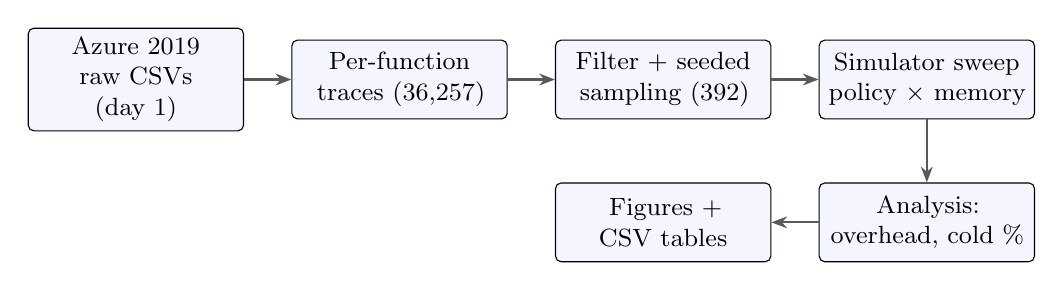
\begin{tikzpicture}[
  box/.style={draw, rounded corners=2pt, align=center, font=\small, minimum height=1.0cm, text width=2.5cm, fill=blue!4},
  arr/.style={-{Stealth[length=2mm]}, thick, gray!70!black}]
  \node[box] (raw)   {Azure 2019\\raw CSVs (day 1)};
  \node[box, right=0.6cm of raw]   (split) {Per-function\\traces (36,257)};
  \node[box, right=0.6cm of split] (samp)  {Filter + seeded\\sampling (392)};
  \node[box, right=0.6cm of samp]  (sim)   {Simulator sweep\\policy $\times$ memory};
  \node[box, below=0.8cm of sim]   (ana)   {Analysis:\\overhead, cold \%};
  \node[box, left=0.6cm of ana]    (fig)   {Figures +\\CSV tables};
  \draw[arr] (raw) -- (split);
  \draw[arr] (split) -- (samp);
  \draw[arr] (samp) -- (sim);
  \draw[arr] (sim) -- (ana);
  \draw[arr] (ana) -- (fig);
\end{tikzpicture}
\caption{Experimental pipeline. Every stage is scripted and resumable; trace sampling is
seeded, so all results are reproducible from the raw dataset (Appendix~\ref{app:repro}).}
\label{fig:pipeline}
\end{figure}

% ===========================================================================
\section{Pitfalls in Reproducing the Artifact}
\label{sec:pitfalls}

Two problems in the published artifact each invalidate a naive reproduction without raising
any error. We describe them because they are easy to fall into and they shaped our methodology.

\subsection{Pitfall 1: a trace that no server can hold}
\label{sec:pitfall-trace}
Our first sweep used a 392-function representative trace sampled \emph{without} the footprint
filter. Every policy produced nearly the same result at every memory size, and between 87\%
and 97\% of all requests were dropped even at 24\,GB (Table~\ref{tab:pathology}).

The cause is the combination of three properties of the simulator and trace: running
containers cannot be evicted; every concurrent request needs its own container; and a cold
start runs for the function's \emph{maximum} recorded duration. A single sampled function
(51\,MB per container, about 20 requests per second, 81-second average duration) needed about
1,600 concurrently running containers --- roughly 80\,GB --- on its own. Such a function pins
all available memory with containers that no policy is allowed to evict, so the keep-alive
policy has nothing to decide and every policy looks identical.

Filtering on \emph{average} duration removed that function but still left about half of all
requests dropped at 16\,GB. The remaining culprit is \emph{cold-start cascades}: for a busy
function whose maximum duration is hundreds of times its average (e.g.\ 56\,s versus 142\,ms),
one cold start keeps a container busy for the full maximum duration, and every arrival during
that time also misses and starts another long-running cold container. Filtering on the cold-start
burst (Equation~\eqref{eq:filter}) removes both effects; with it, requests are dropped only when
memory is genuinely scarce, and the policies separate cleanly.

\begin{table}[H]
\centering
\caption{Percentage of requests dropped under \gd{} for three versions of the trace.
The first two rows used the 12:00--14:00 window of an earlier sample; the last row is the
final full-day trace \code{392-a}.}
\label{tab:pathology}
\begin{tabular}{@{}lccccc@{}}
\toprule
\textbf{Trace version} & \textbf{2\,GB} & \textbf{4\,GB} & \textbf{8\,GB} & \textbf{16\,GB} & \textbf{24\,GB} \\
\midrule
No filter (2-hour window)                   & --      & --     & --     & --     & 86.8\% \\
Filter on average duration (2-hour window)  & --      & 85.9\% & 76.0\% & 53.2\% & -- \\
Filter on cold-start burst, Eq.~\eqref{eq:filter} (full day) & 22.1\% & 5.7\% & 0.3\% & 0.0\% & -- \\
\bottomrule
\end{tabular}
\end{table}

\textbf{Lesson:} when every policy looks identical, the first thing to check is the
dropped-request count, not the policy code.

\subsection{Pitfall 2: an inverted latency metric}
\label{sec:pitfall-metric}
The artifact's analysis script computes a per-function ``percentage increase in execution
time'' as
\[
  \frac{w_f \cdot \mathit{misses}_f}{(\mathit{misses}_f + \mathit{hits}_f)\,(r_f - w_f)},
\]
that is, it treats the warm time $w_f$ as the cold-start \emph{penalty} and $r_f - w_f$ as
the normal execution time. The simulator does the opposite: a warm hit takes $w_f$ and a cold
start takes $r_f$, so the penalty per cold start is $r_f - w_f$ --- which is also the cost term
\gd{} itself uses. On our traces the artifact's metric is dominated by a few functions whose
maximum duration is close to their average, where its ratio becomes very large; it produced a
flat floor of about 18\% that did not decrease with memory even as cold starts fell below 2\%,
and a spurious sudden drop for one policy. We therefore report cold-start overhead
(Equation~\eqref{eq:overhead}), which uses the simulator's own definition. Our cold-start
percentage was cross-checked against the artifact's analysis over all 112 baseline simulations
and agrees to within 0.001 percentage points.

% ===========================================================================
\section{Reproduction Results}
\label{sec:baseline}

\subsection{Cold-start overhead}
Figure~\ref{fig:overhead} shows total cold-start overhead for all seven policies on trace
\code{392-a}, and Table~\ref{tab:baseline} lists selected values.

\begin{figure}[H]
\centering
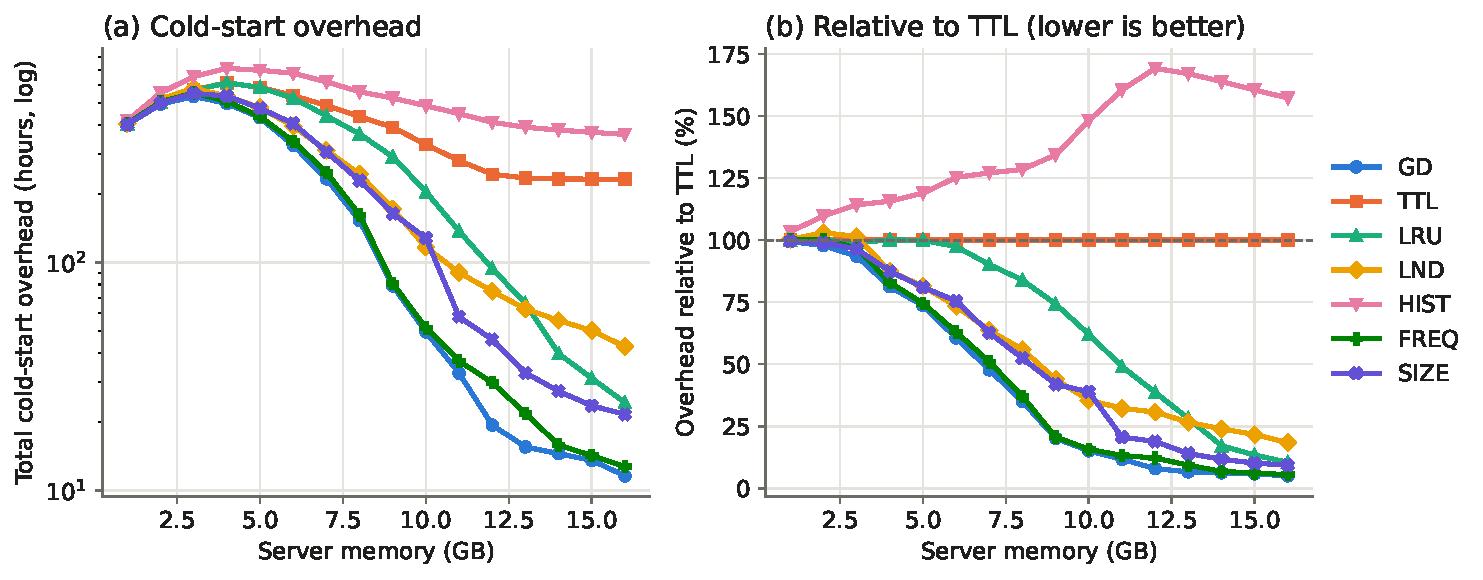
\includegraphics[width=\linewidth]{overhead_mem-392.pdf}
\caption{Cold-start overhead versus server memory on trace \code{392-a}: (a) absolute
(log scale), (b) relative to TTL. \gd{} has the lowest overhead at every memory size from
3\,GB upwards.}
\label{fig:overhead}
\end{figure}

\begin{table}[H]
\centering
\caption{Cold-start overhead (hours) on trace \code{392-a}, and the ratio to \gd{} in parentheses.}
\label{tab:baseline}
\begin{tabular}{@{}lrrrr@{}}
\toprule
\textbf{Policy} & \textbf{4\,GB} & \textbf{8\,GB} & \textbf{12\,GB} & \textbf{16\,GB} \\
\midrule
\gd{}  & 499.1 \phantom{(0.00$\times$)} & 152.7 \phantom{(0.00$\times$)} & 19.3 \phantom{(00.0$\times$)} & 11.6 \phantom{(00.0$\times$)} \\
FREQ   & 509.5 (1.02$\times$) & 161.8 (1.06$\times$) & 29.7 (1.54$\times$)  & 12.7 (1.10$\times$) \\
SIZE   & 537.2 (1.08$\times$) & 228.8 (1.50$\times$) & 45.9 (2.37$\times$)  & 21.6 (1.86$\times$) \\
LND    & 537.5 (1.08$\times$) & 244.3 (1.60$\times$) & 74.8 (3.87$\times$)  & 42.8 (3.69$\times$) \\
LRU    & 615.2 (1.23$\times$) & 366.4 (2.40$\times$) & 94.2 (4.87$\times$)  & 24.3 (2.10$\times$) \\
TTL    & 614.7 (1.23$\times$) & 437.0 (2.86$\times$) & 243.9 (12.6$\times$) & 232.0 (20.0$\times$) \\
HIST   & 711.0 (1.42$\times$) & 561.3 (3.68$\times$) & 412.6 (21.3$\times$) & 364.9 (31.5$\times$) \\
\bottomrule
\end{tabular}
\end{table}

\paragraph{\gd{} versus TTL.} At 8\,GB, \gd{}'s cold-start overhead is $2.9\times$ lower than
TTL's, matching FaasCache's headline claim of roughly $3\times$. The gap widens with memory:
TTL's fixed 10-minute timeout keeps evicting containers that have been idle for 10 minutes even
when memory is free, so its overhead plateaus at about 230 hours, while \gd{} keeps expensive
containers as long as memory allows and its overhead keeps falling.

\paragraph{Ranking.} At 8\,GB the ordering is
\gd{} $<$ FREQ $<$ SIZE $<$ LND $<$ LRU $<$ TTL $<$ HIST;
the middle of the ranking shifts with memory (e.g.\ LRU overtakes LND at 16\,GB), but \gd{} is
best and TTL and HIST are worst throughout.
This is what the caching analogy predicts: policies that account for cold-start cost
(\gd{}, FREQ, LND) do best, recency alone (LRU) is weaker, and a cost-blind timeout (TTL) is
weakest. FREQ --- \gd{} without the size term --- comes close to \gd{} at moderate memory but
falls clearly behind at 12\,GB ($1.54\times$), so the size term is not redundant.

\paragraph{HIST.} The histogram policy is the worst on this trace, with up to $31\times$ the
overhead of \gd{}. Its per-function keep-alive windows are learned from inter-arrival times,
and pre-warmed containers are discarded after use. A likely explanation, which we did not
investigate further, is that on a trace whose functions have long and highly variable
execution times this often discards exactly the containers that are expensive to restart.

\subsection{Cold starts and dropped requests}
\begin{figure}[H]
\centering
\begin{minipage}{0.49\linewidth}
  \centering
  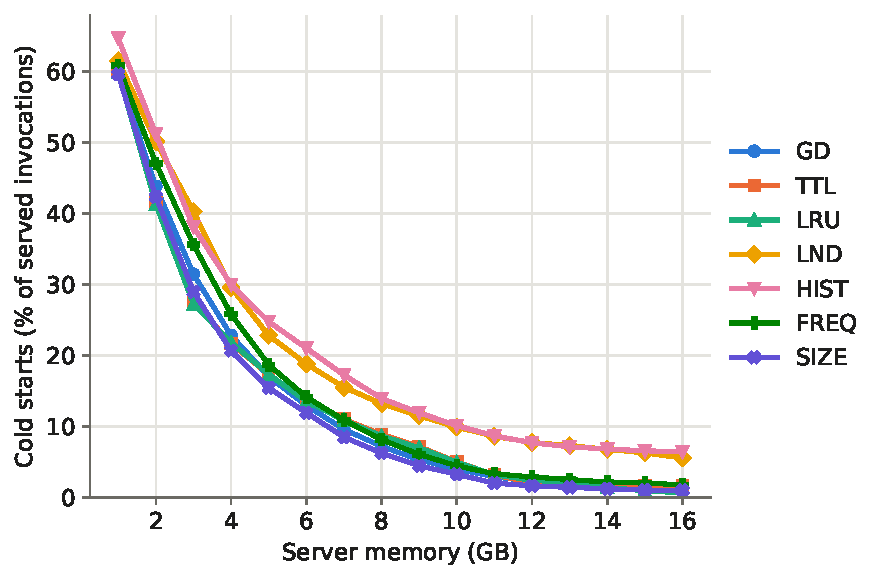
\includegraphics[width=\linewidth]{cold_pct_mem-392.pdf}
\end{minipage}\hfill
\begin{minipage}{0.49\linewidth}
  \centering
  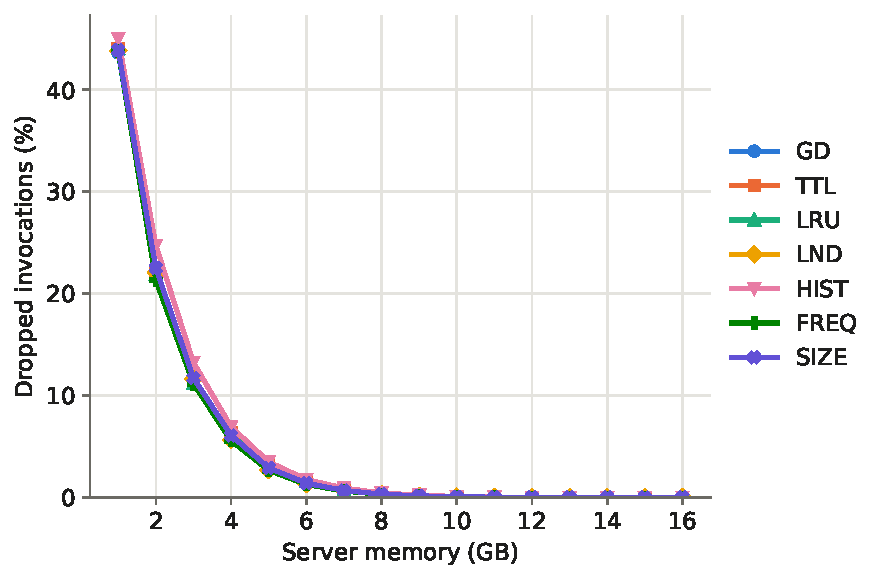
\includegraphics[width=\linewidth]{dropped_mem-392.pdf}
\end{minipage}
\caption{Left: cold starts as a percentage of served invocations. Right: percentage of
invocations dropped because no container could be created. Trace \code{392-a}.}
\label{fig:coldpct}
\end{figure}

Figure~\ref{fig:coldpct} (left) shows an important subtlety: by the \emph{number} of cold
starts, \gd{} is not the best policy. SIZE has fewer cold starts at every memory size from 4\,GB
(e.g.\ 6.2\% versus 7.2\% at 8\,GB), and TTL is within about two percentage points of \gd{}
(8.9\% at 8\,GB, and fewer than \gd{} at some sizes). But
SIZE has $1.5\times$ \gd{}'s overhead at 8\,GB, and TTL $2.9\times$. Fewer cold starts is not
the same as less cold-start time: \gd{} deliberately accepts cold starts on cheap functions to
avoid them on expensive ones. This trade-off is central to our extension results as well
(Section~\ref{sec:mechanism}).

Figure~\ref{fig:coldpct} (right) shows that dropped requests are significant only below
about 4\,GB (22\% at 2\,GB, 6\% at 4\,GB), where all policies thrash and converge, and are
essentially zero from 8\,GB. Because dropped requests incur no cold-start time,
overhead in Figure~\ref{fig:overhead}(a) actually \emph{rises} from 1 to 4\,GB as fewer
requests are dropped and more are served cold.

\subsection{Robustness across trace samples}
\label{sec:baseline-seeds}
A single sampled trace could favour \gd{} by chance. We therefore repeated the comparison on
two further independently sampled traces (\code{392-b}, \code{392-c}), normalising each
policy's overhead by \gd{}'s on the same trace so that differences in workload size cancel.

\begin{figure}[H]
\centering
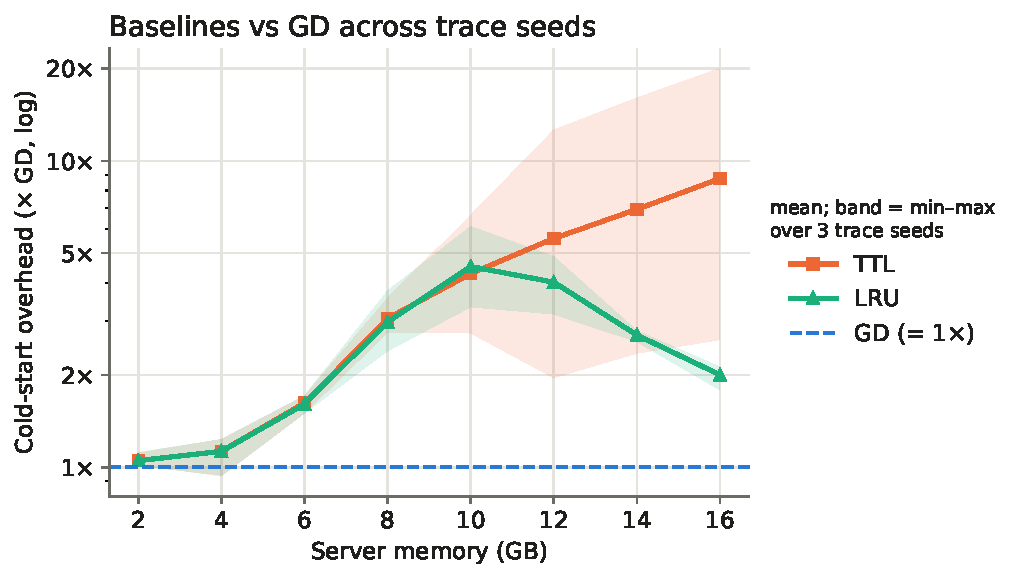
\includegraphics[width=0.78\linewidth]{baseline_vs_gd-392.pdf}
\caption{TTL and LRU cold-start overhead as a multiple of \gd{}'s, mean (line) and
min--max (band) over three trace seeds. Log scale.}
\label{fig:baselineseeds}
\end{figure}

Figure~\ref{fig:baselineseeds} confirms that the reproduction is robust: at 8\,GB, TTL's
overhead is $3.1\times$ \gd{}'s on average (range $2.8$--$3.6\times$ across seeds), and by
16\,GB it is $8.8\times$ on average. LRU tracks TTL up to 10\,GB and then partly recovers
($2.0\times$ at 16\,GB), because without a timeout it eventually keeps everything when memory
is plentiful. The only exception is at 4\,GB on seed \code{b}, where TTL and LRU have about 6\%
less overhead than \gd{}; at such low memory every policy thrashes and \gd{}'s advantage is not
guaranteed.

% ===========================================================================
\section{Extension: Variants of Greedy-Dual}
\label{sec:extension}

\subsection{Motivation}
Equation~\eqref{eq:gd} combines three terms with equal, fixed weight, and its frequency term
has two notable properties in the simulator's implementation: it is a running count that never
decays while a function's containers stay warm, and it is \emph{in-cache} only --- it is the
sum of access counts of the function's live containers, so it resets to zero when all of a
function's containers are evicted. The paper's own FREQ and SIZE baselines are Equation~\eqref{eq:gd}
with one term removed, which suggests a natural family of generalisations. We designed three
variants, each changing exactly one aspect of how \gd{} uses frequency and cost:

\begin{table}[H]
\centering
\caption{The three extension variants.}
\label{tab:variants}
\begin{tabular}{@{}llp{7.2cm}@{}}
\toprule
\textbf{Variant} & \textbf{Changes} & \textbf{Priority} \\
\midrule
\gdw{} & weighting of the terms & $\mathit{Clock} + \mathit{Freq}^{a}\cdot\mathit{Cost}^{b}/\mathit{Size}^{c}$ \\
\gdd{} & age of the frequency information & as \gd{}, with each container's count decayed by $e^{-\Delta t/\tau}$ \\
\gdh{} & where frequency is kept & as \gd{}, with a per-function count that survives eviction \\
\bottomrule
\end{tabular}
\end{table}

\paragraph{\gdw{} (weighted exponents).} $\gd{} = \gdw(1,1,1)$, FREQ $= \gdw(1,1,0)$ and SIZE
$= \gdw(1,0,1)$, so the paper's baselines are fixed points of this family. Sweeping $(a,b,c)$
asks whether the paper's equal weighting is actually the best choice.

\paragraph{\gdd{} (frequency decay).} Each container keeps an exponentially decayed access
count $\phi \leftarrow \phi\, e^{-\Delta t/\tau} + 1$, updated on access and decayed to the
current time whenever a priority is computed. A function that was popular hours ago but is now
quiet thus loses its frequency advantage. The hypothesis is that the trace's strong time-of-day
patterns make stale popularity harmful.

\paragraph{\gdh{} (persistent frequency).} The scheduler keeps a per-function access count
that is \emph{not} reset when the function's containers are evicted (optionally also decayed
with time constant $\tau$). A popular function that loses its containers during a memory
crunch then returns with its history rather than with frequency~1. This is the classic
in-cache versus global frequency question in caching, as in TinyLFU's use of frequency
information beyond the cache's contents~\cite{einziger2017tinylfu}.

\subsection{Implementation and validation}
All three variants are implemented in the simulator's scheduler (about 70 lines, mostly in
its priority function). Their
parameters are encoded in the policy name (e.g.\ \code{GDW\_a1\_b2\_c1}, \code{GDD\_t120},
\code{GDH}), so the existing sweep, analysis and plotting pipeline works unchanged. Before any
large experiment we validated the implementation on a 20-function trace (355,229 invocations)
at 256, 512 and 1024\,MB, where thousands of evictions occur:
\begin{itemize}
  \item \code{GDW\_a1\_b1\_c1} reproduces \gd{} \emph{exactly} --- identical per-function hits,
        misses, evictions and dropped requests;
  \item \gdd{} with $\tau \to \infty$ ($10^9$ minutes) reproduces \gd{} exactly;
  \item \gdh{}'s per-function count equals the total number of served invocations of every
        function, across up to 6,205 evictions per run, confirming that it survives eviction;
  \item short time constants and \gdh{} measurably change behaviour.
\end{itemize}
In addition, \code{GDW\_a1\_b1\_c0} reproduced the simulator's independent FREQ implementation
exactly on the full trace (Table~\ref{tab:screen}). Any difference between a variant and \gd{}
is therefore due to its parameters, not to implementation error.

\subsection{Evaluation protocol}
To keep the compute budget manageable we used a two-stage protocol:
\begin{enumerate}
  \item \textbf{Screening}: 16 variant configurations on trace \code{392-a} at 4, 8 and 12\,GB
        (48 simulations).
  \item \textbf{Confirmation}: the best configuration of each family, together with \gd{}, TTL,
        LRU and FREQ, on all three trace seeds at 2--16\,GB in 2\,GB steps (168 simulation
        results). Each variant is compared to \gd{} on the \emph{same} trace and memory size,
        and we count on how many seeds it beats \gd{}.
\end{enumerate}

% ===========================================================================
\section{Extension Results}
\label{sec:extresults}

\subsection{Screening}
\begin{table}[H]
\centering
\caption{Screening on trace \code{392-a}: cold-start overhead as a percentage of \gd{}'s
(below 100 = better than \gd{}). Sorted by mean.}
\label{tab:screen}
\small
\begin{tabular}{@{}llrrrr@{}}
\toprule
\textbf{Configuration} & \textbf{Meaning} & \textbf{4\,GB} & \textbf{8\,GB} & \textbf{12\,GB} & \textbf{Mean} \\
\midrule
\code{GDW\_a1\_b2\_c1}     & cost squared              & 98.5  & 95.2  & 99.8  & \textbf{97.8} \\
\code{GDW\_a0.5\_b1\_c1}   & frequency square-rooted   & 97.5  & 95.6  & 102.2 & 98.4 \\
\code{GDW\_a0.5\_b1\_c0.5} &                           & 97.7  & 97.2  & 100.6 & 98.5 \\
\code{GDH}                 & persistent frequency      & 98.7  & 96.3  & 101.5 & 98.8 \\
\code{GDW\_a1\_b1\_c0.5}   & size square-rooted        & 99.8  & 98.5  & 105.1 & 101.1 \\
\code{GDD\_t120}           & decay, $\tau=120$\,min    & 99.1  & 98.8  & 107.1 & 101.7 \\
\code{GDH\_t120}           & persistent + decay        & 100.1 & 101.2 & 104.7 & 102.0 \\
\code{GDW\_a0.5\_b1\_c0}   &                           & 100.6 & 101.3 & 104.7 & 102.2 \\
\code{GDD\_t30}            & decay, $\tau=30$\,min     & 100.1 & 101.3 & 105.5 & 102.3 \\
\code{GDH\_t30}            & persistent + decay        & 100.6 & 103.1 & 106.5 & 103.4 \\
\code{GDD\_t5}             & decay, $\tau=5$\,min      & 99.6  & 107.9 & 105.6 & 104.3 \\
\code{GDW\_a1\_b0.5\_c1}   & cost square-rooted        & 101.2 & 117.5 & 115.1 & 111.3 \\
\code{GDW\_a2\_b1\_c1}     & frequency squared         & 102.7 & 119.8 & 121.1 & 114.5 \\
\code{GDW\_a1\_b1\_c0}     & = FREQ (no size term)     & 102.1 & 105.9 & 153.5 & 120.5 \\
\code{GDW\_a2\_b1\_c0.5}   &                           & 103.6 & 120.0 & 161.6 & 128.4 \\
\code{GDW\_a2\_b1\_c0}     &                           & 106.8 & 127.3 & 172.7 & 135.6 \\
\midrule
TTL                        & reference                 & 123.2 & 286.2 & 1260.6 & 556.6 \\
\bottomrule
\end{tabular}
\end{table}

Table~\ref{tab:screen} shows clear and consistent patterns:
\begin{itemize}
  \item \textbf{Weighting.} Putting more weight on cost ($b=2$) or less on frequency ($a=0.5$)
        helps; putting more weight on frequency ($a=2$) hurts by 15--20\%; weakening the cost
        term ($b=0.5$) hurts by about 11\%. Removing the size term ($c=0$) hurts most, and
        most at higher memory (up to 73\% worse at 12\,GB). \gd{}'s equal weighting is close
        to, but not exactly at, the best point in this family.
  \item \textbf{Decay.} Every decayed variant is worse than its undecayed counterpart, and
        shorter time constants are worse ($\tau = 5 > 30 > 120$ minutes, for both \gdd{} and
        decayed \gdh{}). Old popularity remains informative on this trace.
  \item \textbf{Persistence.} Plain \gdh{} looked promising (2--4\% better at 4--8\,GB).
\end{itemize}
We carried the best configuration of each family --- \code{GDW\_a1\_b2\_c1}, \code{GDH} and
\code{GDD\_t120} --- forward to confirmation.

\subsection{Confirmation across three trace seeds}
\begin{figure}[H]
\centering
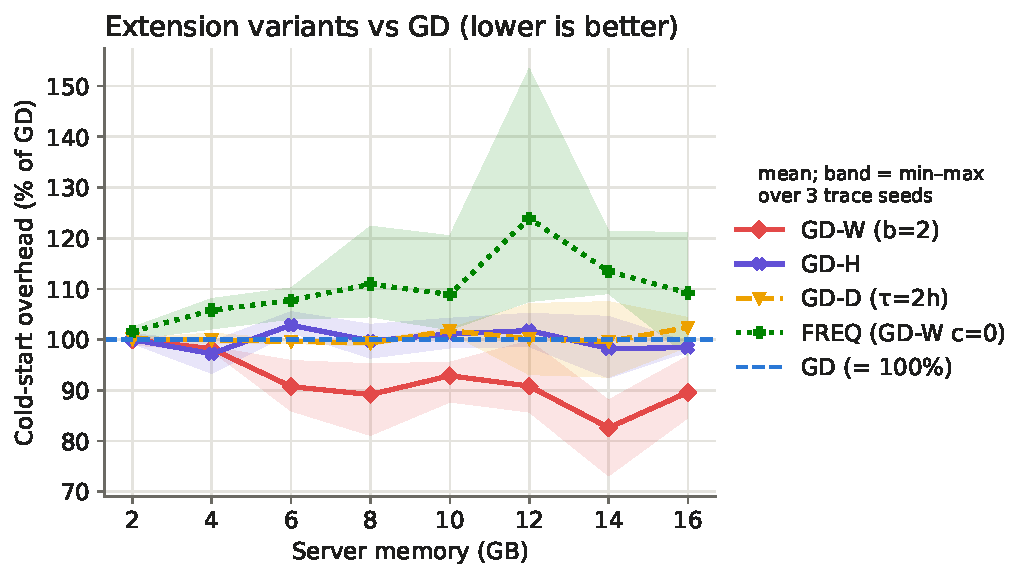
\includegraphics[width=0.85\linewidth]{ext_vs_gd-392.pdf}
\caption{Cold-start overhead of the extension variants (and FREQ) as a percentage of \gd{}'s,
mean (line) and min--max (band) over three trace seeds. Below the dashed line is better than
\gd{}.}
\label{fig:extseeds}
\end{figure}

\begin{table}[H]
\centering
\caption{Cold-start overhead as a percentage of \gd{}'s: mean over three seeds, and the number
of seeds on which the variant beats \gd{}.}
\label{tab:seeds}
\small
\resizebox{\linewidth}{!}{%
\setlength{\tabcolsep}{4.5pt}
\begin{tabular}{@{}lcccccccc@{}}
\toprule
\textbf{Variant} & \textbf{2\,GB} & \textbf{4\,GB} & \textbf{6\,GB} & \textbf{8\,GB} & \textbf{10\,GB} & \textbf{12\,GB} & \textbf{14\,GB} & \textbf{16\,GB} \\
\midrule
\gdw{} ($b{=}2$) & 99.9 (2/3) & \textbf{98.2} (3/3) & \textbf{90.7} (3/3) & \textbf{89.1} (3/3) & \textbf{92.9} (3/3) & \textbf{90.8} (3/3) & \textbf{82.6} (3/3) & \textbf{89.6} (3/3) \\
\gdh{}           & 100.0 (2/3) & 97.2 (3/3) & 102.8 (0/3) & 99.7 (2/3) & 101.1 (1/3) & 101.8 (1/3) & 98.2 (2/3) & 98.4 (3/3) \\
\gdd{} ($\tau{=}2$h) & 100.1 (1/3) & 99.9 (2/3) & 99.6 (3/3) & 99.3 (3/3) & 101.8 (0/3) & 100.1 (1/3) & 99.6 (2/3) & 102.4 (1/3) \\
FREQ             & 101.6 (0/3) & 105.8 (0/3) & 107.7 (0/3) & 110.9 (0/3) & 108.9 (0/3) & 123.9 (0/3) & 113.4 (0/3) & 109.2 (1/3) \\
\bottomrule
\end{tabular}}
\end{table}

Figure~\ref{fig:extseeds} and Table~\ref{tab:seeds} give the main extension result:
\begin{itemize}
  \item \textbf{\gdw{} with a squared cost term beats \gd{} on every seed at every memory size
        from 4\,GB to 16\,GB} (21 of 21 seed--memory combinations), reducing cold-start
        overhead by 9--17\% at 6--16\,GB (best: 82.6\% of \gd{} at 14\,GB, range 73--88\%).
        At 2\,GB, where every policy thrashes, it ties with \gd{}. On trace \code{392-b} the
        improvement is even larger than on \code{392-a}, where it was selected (81\% of \gd{}
        at 8\,GB), so it is not an artefact of screening on one trace.
  \item \textbf{\gdh{} shows no reliable effect.} Its 2--4\% gain on \code{392-a} did not
        replicate: across seeds it lands between 97\% and 103\% of \gd{}, on both sides
        depending on seed and memory size. This illustrates why screening results on a single
        trace must be confirmed before they are reported.
  \item \textbf{\gdd{} is neutral to slightly worse} (99--102\% of \gd{}), consistent with
        screening: decaying frequency does not help on this workload.
  \item \textbf{FREQ is worse than \gd{} at every memory size} (106--124\%), on essentially
        every seed: re-weighting the size term can help, but removing it hurts.
\end{itemize}

% ===========================================================================
\section{Why GD-W Works: A Count-for-Cost Trade-off}
\label{sec:mechanism}

To understand \gdw{}'s improvement we split each trace's functions into quartiles by cold-start
cost $c_f = r_f - w_f$ and compared \gdw{} with \gd{} within each quartile
(Figure~\ref{fig:mechanism}, Table~\ref{tab:mechanism}).

\begin{figure}[H]
\centering
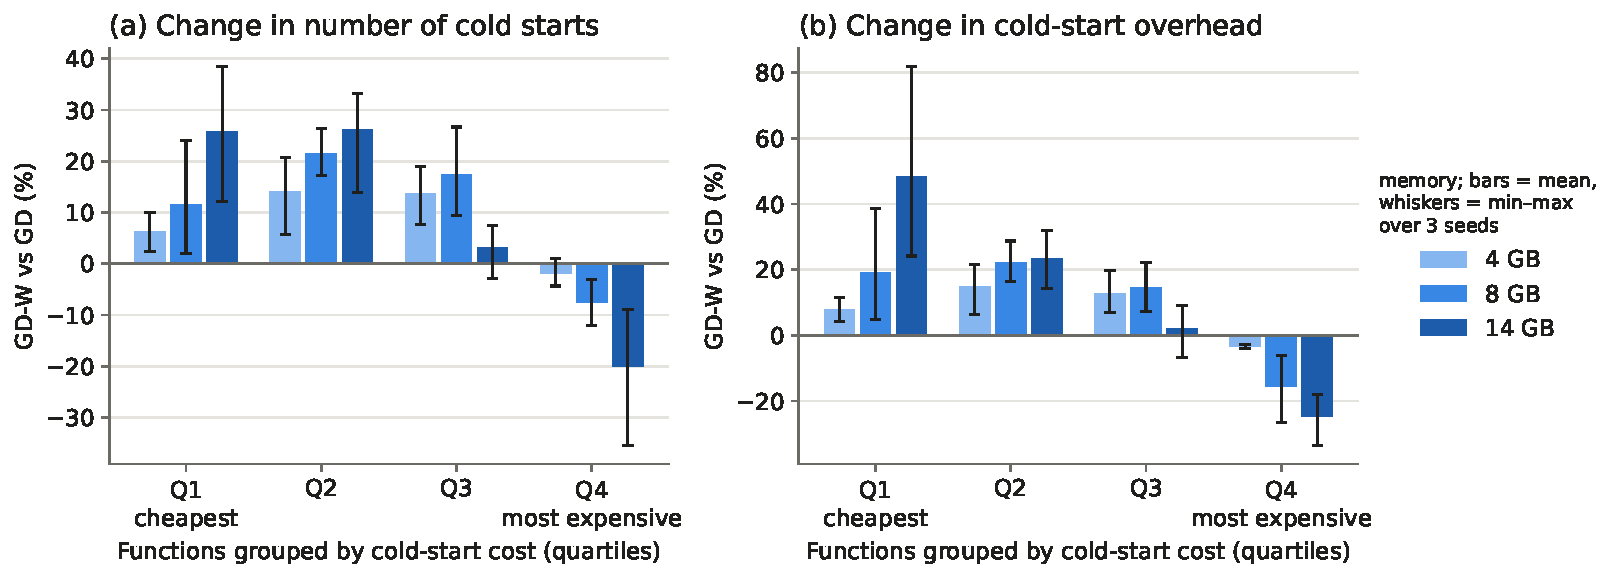
\includegraphics[width=\linewidth]{gdw_mechanism-392.pdf}
\caption{\gdw{} ($b{=}2$) versus \gd{}, by cold-start-cost quartile: (a) change in the number
of cold starts, (b) change in cold-start overhead. Bars show the mean over three seeds,
whiskers the min--max.}
\label{fig:mechanism}
\end{figure}

\begin{table}[H]
\centering
\caption{\gdw{} versus \gd{} per cost quartile (mean over three seeds). ``Share'' is the
quartile's fraction of \gd{}'s total cold-start overhead.}
\label{tab:mechanism}
\small
\resizebox{\linewidth}{!}{%
\begin{tabular}{@{}l rrr rrr rrr@{}}
\toprule
 & \multicolumn{3}{c}{\textbf{4\,GB}} & \multicolumn{3}{c}{\textbf{8\,GB}} & \multicolumn{3}{c}{\textbf{14\,GB}} \\
\cmidrule(lr){2-4}\cmidrule(lr){5-7}\cmidrule(l){8-10}
\textbf{Quartile} & share & $\Delta$cold & $\Delta$ovh & share & $\Delta$cold & $\Delta$ovh & share & $\Delta$cold & $\Delta$ovh \\
\midrule
Q1 (cheapest)        & 0.2\%  & $+6.3\%$  & $+7.9\%$  & 0.5\%  & $+11.6\%$ & $+19.0\%$ & 1.5\%  & $+25.7\%$ & $+48.4\%$ \\
Q2                   & 1.6\%  & $+14.1\%$ & $+14.8\%$ & 3.0\%  & $+21.6\%$ & $+22.1\%$ & 5.9\%  & $+26.2\%$ & $+23.3\%$ \\
Q3                   & 8.0\%  & $+13.8\%$ & $+12.8\%$ & 10.3\% & $+17.5\%$ & $+14.6\%$ & 12.9\% & $+3.1\%$  & $+1.9\%$ \\
Q4 (most expensive)  & 90.2\% & $-2.0\%$  & $-3.4\%$  & 86.2\% & $-7.5\%$  & $-15.6\%$ & 79.7\% & $-20.0\%$ & $-24.8\%$ \\
\midrule
\textbf{All}         & 100\%  & $+7.0\%$  & $\mathbf{-1.8\%}$ & 100\% & $+11.8\%$ & $\mathbf{-10.9\%}$ & 100\% & $+18.9\%$ & $\mathbf{-17.4\%}$ \\
\bottomrule
\end{tabular}}
\end{table}

The breakdown explains the result:
\begin{enumerate}
  \item \textbf{Cold-start time is highly concentrated.} The most expensive quartile of
        functions carries 80--90\% of \gd{}'s total cold-start overhead; the cheapest quartile
        carries under 2\%. (This follows from the heavy tail of maximum durations in the
        Azure trace.)
  \item \textbf{\gdw{} protects that quartile much more strongly.} Squaring the cost term
        widens the priority gap between expensive and cheap functions, so \gdw{} evicts expensive
        containers less often: Q4's cold starts fall by up to 20\% and its overhead by up to 25\%,
        on every seed.
  \item \textbf{It pays with more cold starts on cheap functions.} Q1--Q3 see 3--26\% more cold
        starts, and the \emph{total number} of cold starts rises by 7--19\%.
  \item \textbf{The trade is favourable for total latency.} Because each saved cold start is
        expensive and each extra one is cheap, total overhead falls by 2--17\%, growing with
        memory as there is more room to protect expensive containers.
\end{enumerate}

\gdw{} therefore \emph{trades cold-start count for cold-start time}. This is the right trade
when the objective is total cold-start latency --- the objective used by FaasCache and by us ---
but the wrong one if a provider cares about the cold-start \emph{rate}, or about the tail latency
of cheap, latency-sensitive functions. The cost exponent $b$ is best understood as a policy knob
that sets where a platform sits on this trade-off, rather than as a strictly better
algorithm. The same trade-off already separates \gd{} from SIZE and TTL in the baseline
(Section~\ref{sec:baseline}): \gdw{} simply pushes further along it.

% ===========================================================================
\section{Discussion}
\label{sec:discussion}

\paragraph{The caching analogy holds up.} On a real production workload, cost-aware caching
policies dominate recency-only and timeout-based keep-alive, by a margin that grows with
available memory. The most important single ingredient is the cost term: every configuration
that weakens it performs worse, and strengthening it is the one change that robustly helps.

\paragraph{Why decay and persistence did not help.} Both \gdd{} and \gdh{} target the frequency
term, and both turned out neutral. A likely reason is that \gd{}'s $\mathit{Clock}$ already
provides ageing: a container that is not accessed keeps its old priority while the clock rises
past it, so long-idle containers are evicted regardless of their past frequency. Additional
decay therefore mostly penalises functions that are still active, and the screening shows that
shorter decay is consistently worse. Similarly, frequency only differs between \gd{} and \gdh{}
for functions that are completely evicted and later return, which at moderate memory are mostly
infrequent functions whose history is short anyway.

\paragraph{Negative results matter.} \gdh{} looked like a 2--4\% improvement after screening on
one trace and would have been reported as such without the multi-seed confirmation. Normalising
by \gd{} on the same trace and counting the seeds on which a variant wins proved to be a simple
and effective guard against such false positives.

\paragraph{Reproducing research artifacts.} Both pitfalls in Section~\ref{sec:pitfalls} produce
plausible-looking output with no errors: identical curves that could be mistaken for ``the
policies don't matter on this trace'', and a latency metric that looks reasonable in isolation.
Both were found only by checking intermediate quantities (dropped requests; per-function
contributions to the metric) rather than final plots.

% ===========================================================================
\section{Threats to Validity and Limitations}
\label{sec:limitations}

\begin{itemize}
  \item \textbf{Trace construction.} Following the artifact, invocations are spread evenly
        within each minute, memory is the application average divided among its functions,
        and the cold-start time is the \emph{maximum} recorded duration. The latter makes
        cold starts very expensive for functions with heavy-tailed durations, and amplifies
        the benefit of cost-aware policies at high memory. Absolute overhead values should
        therefore be read relative to one another, not as real latencies.
  \item \textbf{Footprint filter.} Excluding functions whose cold-start burst exceeds 2\,GB
        removes the largest 5.5\% of functions (about 93\% of invocations). This is necessary
        for the comparison to be meaningful on a single server, but it means our results
        describe the remaining 94.5\% of functions, not the very busiest ones.
  \item \textbf{Simulation, not a real platform.} The simulator assumes unlimited CPU, no
        queueing, and drops requests that cannot be placed. We did not run the OpenWhisk-based
        real-system experiments of the original paper.
  \item \textbf{Workload coverage.} We use one day of one provider's trace, and the
        representative sampling only; the paper's RARE and RANDOM trace variants were not
        evaluated. Results are confirmed on three independently sampled traces, but three
        samples bound the variability only coarsely.
  \item \textbf{Metric.} \gdw{}'s improvement is in total cold-start time; it increases the
        number of cold starts (Section~\ref{sec:mechanism}). Under a cold-start-rate or
        tail-latency objective it would not be an improvement.
\end{itemize}

% ===========================================================================
\section{Future Work}
\label{sec:future}
\begin{itemize}
  \item \textbf{Other workloads}: evaluate \gdw{} on the RARE and RANDOM traces and on other
        days of the Azure dataset, to test whether the optimal cost exponent is workload-dependent.
  \item \textbf{Tuning $b$ online}: adapt the cost exponent to an explicit objective (e.g.\ a
        weighted combination of cold-start time and cold-start rate) or to observed workload.
  \item \textbf{Clone-aware eviction}: all warm containers of one function share a priority, so
        a function that briefly scaled out keeps many idle copies at high priority; evicting
        surplus copies first is a promising refinement.
  \item \textbf{Admission control}: a ``doorkeeper'' that does not keep the container of a
        function's first-ever invocation, as in TinyLFU~\cite{einziger2017tinylfu}.
  \item \textbf{Real-system validation}: implement \gdw{} in a real FaaS platform such as OpenWhisk,
        as the original paper did for \gd{}.
\end{itemize}

% ===========================================================================
\section{Conclusion}
\label{sec:conclusion}
We reproduced FaasCache's central result on the real Azure Functions trace: Greedy-Dual
keep-alive incurs about $3\times$ less cold-start overhead than a fixed 10-minute TTL at 8\,GB
of server memory, and the advantage grows with memory and holds across three independently
sampled traces. Getting there required fixing two silent problems in the published artifact
--- a trace-sampling pathology and an inverted latency metric --- which we documented together
with principled fixes. Extending \gd{} with three variants of its frequency and cost terms,
we found that squaring the cost term (\gdw{}) reduces cold-start overhead by a further 9--17\%,
on every trace and every memory size from 4\,GB upwards, by trading a moderate increase in cheap
cold starts for a substantial reduction in expensive ones. Frequency decay and persistence across
evictions gave no reliable improvement, which we attribute to \gd{}'s clock already providing
effective ageing. Overall, the results strengthen the paper's core message: treating keep-alive as
cost-aware caching works, and the cost of a cold start is the single most important signal for
deciding what to keep warm.

% ===========================================================================
\bibliographystyle{plain}
\bibliography{refs}

% ===========================================================================
\appendix
\section{Reproducibility}
\label{app:repro}

All code, patches and documentation are in the project repository; the simulator patches live on
a separate branch of our fork of the artifact. All commands below are run with the project's
Python virtual environment; full details, timings and troubleshooting notes are in the
repository's \code{WORKFLOW.md}.

\paragraph{1. Trace generation} (from the repository root; raw data in \code{azure-raw-data/}):
\begin{lstlisting}
SPLIT_WORKERS=2 SPLIT_MAX_INVOCATIONS=10000000 \
  python sim-upstream/code/split/gen/trace_split_funcs.py
python sim-upstream/code/split/gen/gen_representative_trace.py --sizes 392 --runs a b c
\end{lstlisting}

\paragraph{2. Baseline sweep} (from \code{sim-upstream/code/split/}; about 25 minutes):
\begin{lstlisting}
python many_run.py --tracedir ../../../experiments/traces/representative \
  --numfuncs 392 --char a --memmin 1000 --memmax 17000 --memstep 1000 \
  --workers 6 --delete-logs \
  --savedir ../../../results/baseline/full_day --logdir ../../../results/baseline/full_day/logs
\end{lstlisting}

\paragraph{3. Extension: tests, screening and multi-seed confirmation.}
\begin{lstlisting}
python experiments/test_gd_variants.py            # exact-equivalence tests
# screening (from sim-upstream/code/split/), then rank:
python many_run.py ... --memmin 4000 --memmax 12001 --memstep 4000 \
  --policies GDW_a1_b2_c1 GDW_a0.5_b1_c1 GDD_t120 GDH ...
python experiments/screen_summary.py results/extension/screen results/baseline/full_day
# confirmation, once per seed (a, b, c):
python many_run.py ... --char b --memmin 2000 --memmax 16001 --memstep 2000 \
  --policies GD TTL LRU FREQ GDW_a1_b2_c1 GDH GDD_t120
\end{lstlisting}

\paragraph{4. Figures and tables} (from the repository root):
\begin{lstlisting}
python experiments/plot_baseline.py --resdir results/baseline/full_day \
  --outdir results/baseline/full_day/figs
python experiments/seed_summary.py --seeds a b c --outdir results/extension/figs
python experiments/gdw_mechanism.py --outdir results/extension/figs
\end{lstlisting}
Each figure script also writes a CSV file with every number behind the figure.

\end{document}
